\documentclass[a4paper,12pt]{article} 
\usepackage[T2A]{fontenc}			
\usepackage[utf8]{inputenc}			
\usepackage[english,russian]{babel}	
\usepackage{amsmath,amsfonts,amssymb,amsthm,mathtools} 
\usepackage[colorlinks, linkcolor = blue]{hyperref}
\usepackage{upgreek}\usepackage[left=2cm,right=2cm,top=2cm,bottom=3cm,bindingoffset=0cm]{geometry}
\usepackage{multirow}
\usepackage{graphicx,wrapfig,lipsum}
\usepackage{xcolor}
\usepackage{pgfplots}


\graphicspath{ {images/} }
\usepackage{multicol}
\setlength{\columnsep}{2cm}

\begin{document}

\begin{titlepage}

\begin{center}
%\vspace*{1cm}
\large\textbf{Московский Физико-Технический Институт}\\
\large\textbf{(государственный университет)}
\vfill
\line(1,0){430}\\[1mm]
\huge\textbf{Измерение магнитного поля Земли}\\
\line(1,0){430}\\[1mm]
\vfill
\large Сибгатуллин Булат, ФРКТ\\
\end{center}

\end{titlepage}
\textbf{Работа 3.1.3}\\
\noindent \textbf{Цель работы:} \\
\indent определить характеристики шарообразных неодимовых магнитов и, используя
законы взаимодействия магнитных моментов с полем, измерить горизонтальную и вертикальную
составляющие индукции магнитного поля Земли и магнитное наклонение.\\
\noindent \textbf{В работе используются:} \\
\indent неодимовые магнитны, тонкая нить для
изготовления крутильного маятника, медная проволока, электронные весы,
секундомер, измеритель магнитной индукции, штангенциркуль, брусок из немагнитного
материала, деревянная линейка, штатив из немагнитного материала;
дополнительные неодимовые магнитные шарики и неодимовые магниты в форме параллелепипедов, набор гирь и разновесов.

\section*{Теория}
\subsection*{Точечный магнитный диполь}
Простейший магнитный диполь может быть образован витком с током или постоянным магнитом. По определению, магнитный момент $\overrightarrow{P_m}$ тонкого витка площадью $S$ с током $I$ равен

\begin{equation}
\overrightarrow{P_m}=\frac{I}{c}\vec{S}=\frac{I}{c}S\vec{n},
\end{equation}

где $\vec{S}=S\vec{n}$ -- вектор площади круга контура. Если размеры контура с током или магнитной стрелки малы по сравнению расстоянием до диполя, то соответствующий магнитный диполь называют элементарным или точечным.\\
Магнитное поле точечного диполя определяется по формуле, аналогичной формуле для поля
элементарного электрического диполя:
\begin{equation}
\vec{B}=\frac{3(\overrightarrow{P_m},\vec{r})\vec{r}}{r^5} - \frac{\overrightarrow{P_m}}{r^3}
\end{equation}

В магнитном поле с индукцией $B$
на точечный магнитный диполь 
действует механический
момент сил:
\begin{equation}
\vec{M} = \overrightarrow{P_m}\times \vec{B}.
\end{equation}

Под действием вращающего момента $\vec{M}$ виток с током или постоянный магнит поворачивается
так, чтобы его магнитный момент выстроился вдоль вектора индукции магнитного поля. Это —
положение устойчивого равновесия: при отклонении от этого положения возникает механический
момент внешних сил, возвращающий диполь к положению равновесия. В положении, когда $\overrightarrow{P_m}$ и $\vec{B}$
параллельны, но направлены противоположно друг другу, также имеет место равновесие ($M$ = 0),
но такое равновесие неустойчиво: малейшее отклонение от этого положения приведёт к появлению
момента сил, стремящихся отклонить диполь ещё дальше от начального положения.\\
Магнитный диполь в магнитном поле обладает энергией:

\begin{equation}
W = -(\overrightarrow{P_m},\vec{B})
\end{equation}

В неоднородном поле на точечный магнитный диполь, кроме момента сил, действует ещё и сила:

\begin{equation}
\vec{F} = (\overrightarrow{P_m} \vec{\triangledown }) \vec{B}
\end{equation}

Используя формулы для момента силы, силы и энергии, не сложно выяснить, как ведёт себя
свободный магнитный диполь в неоднородном магнитном поле: он выстраивается вдоль силовых
линий магнитного поля и, кроме того, под действием результирующей силы, возникающей из-за
неоднородности поля, втягивается в область более сильного магнитного поля, т.е. в область, где он
обладает меньшей энергией.\\
Зная магнитные моменты $P_1 = P_2 = P_m$ двух небольших постоянных магнитов, можно рассчитать силу
их взаимодействия:

\begin{equation}
F = P_m \frac{\partial B}{\partial r}=-6\frac{P_m^2}{r^4}.
\end{equation}

\subsection*{Неодимовые магнитные шары}
В настоящей работе используются неодимовые магниты шарообразной формы.
Для нас важно то, что:\\
1) шары намагничены однородно;\\
2) вещество, из которого изготовлены магниты, является магнитожёстким материалом.\\
Полный магнитный момент $\overrightarrow{P_m}$
постоянного магнита определяется намагниченностью $\overrightarrow{p_m}$
вещества, из которого он изготовлен. По определению, намагниченность – это магнитный момент единицы объёма. Для однородно намагниченного шара намагниченность равна:

\begin{equation}
\overrightarrow{p_m}=\frac{\overrightarrow{P_m}}{V}.
\end{equation}

Намагниченность — важная характеристика вещества постоянных магнитов, определяющая, в
частности, величину остаточной магнитной индукции $B_r = 4\pi p_m$. Индукция магнитного поля $\overrightarrow{B_p}$
на полюсах однородно намагниченного шара связана с величиной намагниченности и остаточной магнитной индукцией формулами

\begin{equation}
\overrightarrow{B_p}=\frac{8\pi}{3}\overrightarrow{p_m}=\frac{2}{3}\overrightarrow{B_r}.
\end{equation}

\section*{Описание работы}
\subsection*{Определение величины магнитного момента магнитных шариков}
\paragraph*{Метод А}
Величину магнитного момента одинаковых шариков
можно рассчитать, зная их массу $m$ и определив максимальное расстояние $r_{max}$, на котором они ещё удерживают друг
друга в поле тяжести. При максимальном расстоянии сила тяжести шариков равна силе их магнитного притяжения:
\begin{center}
$\frac{6P_m^2}{r_{max}^4}=mg\Rightarrow$ \fbox{$P_m = \sqrt{\frac{mgr_{max}^4}{6}}$}
\end{center}
\paragraph*{Метод Б}
Если сила сцепления двух одинаковых шаров диаметром $d$ c магнитными моментами $P_m$ равна:

\begin{equation}
F_0 = \frac{6P_m^2}{d^4}
\end{equation}

то минимальный вес цепочки, при которой она оторвётся от верхнего шарика равен: $F \approx 1.08 F_0$. Тогда\\
\begin{center}
\fbox{$P_m = \sqrt{\frac{Fd^4}{6.48}}$}
\end{center}
\subsection*{Определение величины магнитного поля Земли}
\paragraph*{Горизонтальная составляющая}
\begin{wrapfigure}{R}{3.5cm}
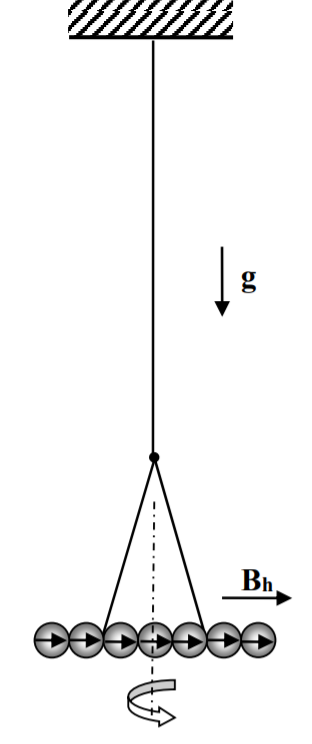
\includegraphics[scale=0.5]{1.png}
\vspace{-60pt}
\end{wrapfigure}  
Магнитная <<стрелка>> образована из $n$ сцепленных друг с другом противоположными полюсами шариков и с помощью $\Lambda$-образного подвеса подвешена в горизонтальном положении. При отклонении «стрелки» на угол $\theta$ от равновесного положения в горизонтальной плоскости возникают крутильные колебания вокруг вертикальной оси, проходящей через середину стрелки. При малых амплитудах уравнение колебаний
стрелки имеет вид:

\begin{equation}
I_n \dfrac{d^2 \theta}{dt^2} + P_0 B_h \theta = 0,
\end{equation}

где $P_0$ -- магнитный момент стрелки, $B_h$ -- горизонтальная составляющая магнитного поля Земли, $I_n \approx \dfrac{1}{12}n^3 m d^3$, тогда период колебаний $T = kn$, где $k = \pi \sqrt{\dfrac{md^2}{3P_m B_h}}$. Измеряя зависимость $T=T(n)$, находится $B_h$:
\begin{center}
\fbox{$B_h = \dfrac{\pi^2 m d^2}{3k^2P_m}$}
\end{center}
\begin{wrapfigure}{R}{6cm}
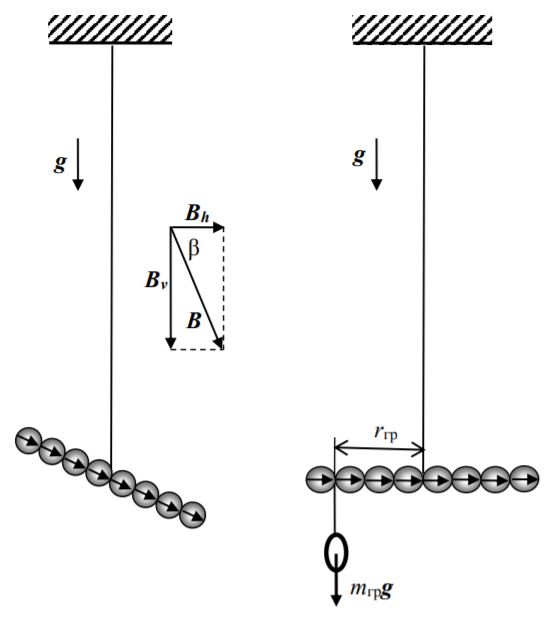
\includegraphics[scale=0.5]{2.png}
\end{wrapfigure} 
\paragraph*{Вертикальная составляющая} 
Магнитная «стрелка», составленная из чётного числа
шариков и подвешенная на тонкой нити за середину, расположится не горизонтально, а под некоторым, отличным от нуля, углом к горизонту. Это связано с тем, что вектор $\vec{B}$ индукции магнитного поля Земли в общем случае не горизонтален, а образует с горизонтом
угол $\beta$, зависящим от географической широты $\varphi$
места, где проводится опыт. Величина угла $\beta$
называется магнитным наклонением.\\
С помощью небольшого дополнительного грузика «стрелку» можно «выровнять». Момент $M$ силы тяжести уравновешивающего груза пропорционален числу $n$ шариков, образующих магнитную «стрелку» $M(n) = An, A=P_m B_v$, то есть
\begin{center}
\fbox{$B_v = \dfrac{A}{P_m}$}
\end{center}

\section*{Ход работы}
\begin{enumerate}
\item Определим вес и диаметр неодимовых магнитов, с помощью весов и штангенциркуля соответственно:

\[M_{\textit{ш}} = 480 \pm 1 \quad \textit{мг}\]

\[d = 2,45 \pm 0,1 \quad \textit{мм}\]

С помощью магнетометра измерим индукцию поля на полюсах шарика:

\[B_p = 22,4 \pm 0,1 \quad \textit{Гс}\]

Определим максимальное расстояние, на котором магниты будут притягиваться (метод А):

\[R_{max} = 14,6 \pm 0,1 \quad \textit{мм} \]

Также определим максимальный вес, который может удерживать магнит (метод Б):

\[M_\textit{г} = 226,426 \pm 0,002 \quad \textit{г}\]

По формулам приведенным в теории найдем намагниченность для методов А и Б:

\[A: \quad M = 309,8 \pm 22,3 \quad \textit{Эрг/(Гс}\cdot \textit{см}^3\textit{)}\]

\[B: \quad M = 728,9 \pm 57,8 \quad \textit{Эрг/(Гс}\cdot \textit{см}^3\textit{)}\]

Вычислим магнитную индукцию:

\[A: \quad 3891 \pm 287 \quad \textit{Гс} \]

\[B: \quad 9156 \pm 734 \quad \textit{Гс} \]

\item В дальнейших измерениях будем использовать значение для магнитной индукции полученной при помощи метода Б. Соберем крутильный маятник используя 12 магнитов свернутых в кольцо. Убедимся, что силу упругости при расчете периода колебаний можно не учитывать.

Исследуем зависимость периода крутильных колебаний от количества магнитных шариков составляющих стрелку. Построим таблицу по получившимся измерениям.

\begin{center}
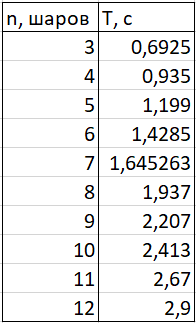
\includegraphics[scale=0.8]{table1.png}
\end{center}

Аналогично соберем магнитную стрелку из четного числа шариков и подвесим ее за середину на штативе. При помощи дополнительных грузиков уравновесим данную стрелку, чтобы она приняла горизонтальное положение. Аналогично проведем измерения для четных значений n = 4, ... , 12. Запишем данные в таблицу.

\begin{center}
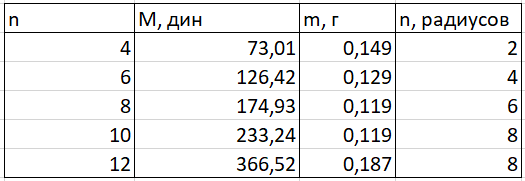
\includegraphics[scale=0.8]{table2.png}
\end{center}

Построим графики зависимости \textit{M(n)} и \textit{T(n)}.

\begin{center}
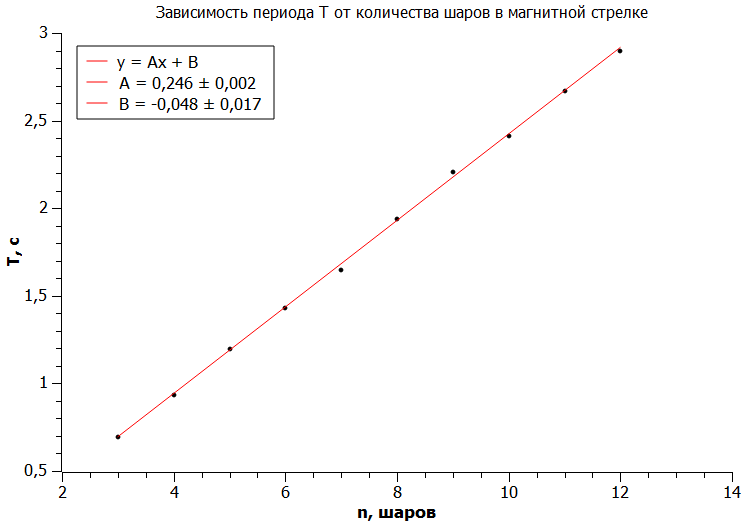
\includegraphics[scale=0.8]{graph1.png}
\end{center}

\begin{center}
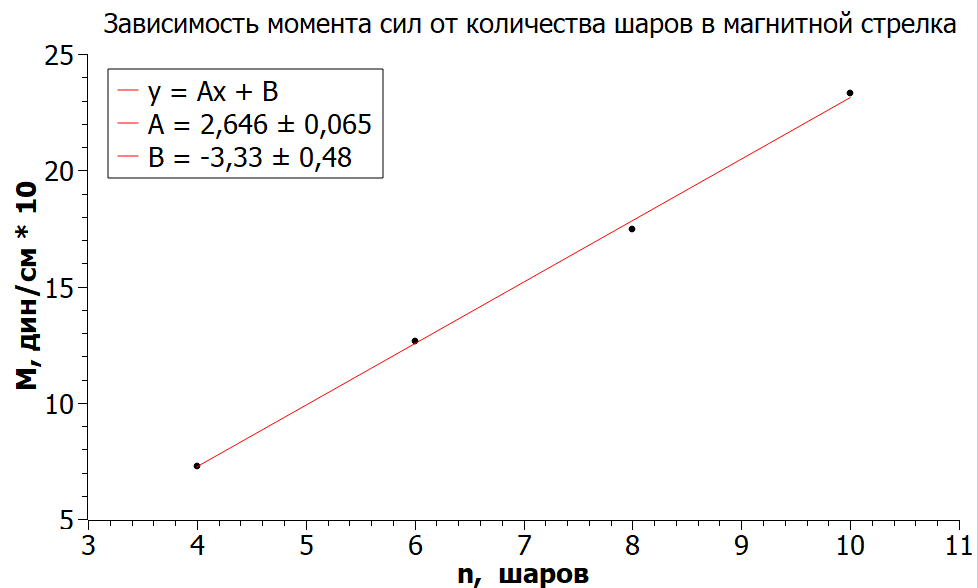
\includegraphics[scale=0.8]{graph2.png}
\end{center}

Зная значения коэффициентов наклона рассчитаем величины $B_{\bot}$ и $B_{\|}$ по формулам:

\[B_{\bot} = \frac{A}{\textbf{m}}\]

\[B_{\|} = \frac{4\pi^2 m R^2}{3\textbf{m} A}\]

Запишем получившиеся значения:

\[B_{\bot} = 0,593 \pm 0,017 \quad \textit{Тл}\]

\[B_{\|} = 0,344 \pm 0,0015 \quad \textit{Тл}\]

Посчитаем значение для магнитного поля и угла:

\[B = 0,681 \pm 0,036 \quad \textit{Гс}\]

\[\beta = 60,1^{\circ} \pm 3,2^{\circ} \]

\section*{Вывод}

Мы вычислили магнитное наклонение и итоговую индукцию магнитного поля. Магнитное поле Земли находится в диапазоне 0,6 - 0,65 \textit{Гс}, что совпадает с нашим значением в пределах погрешности. \\

\end{enumerate}
\end{document}